% Equal heading baselines, matched picture areas, and separate explanatory rows.
\begin{tikzpicture}[remember picture,overlay,
 every node/.style={text=Ink,inner sep=0pt,align=left}]
\begin{scope}[shift={(current page.south west)}]
 \node[anchor=west,font=\normalsize\bfseries] at (.85,7.0)
  {What we want to achieve};
 \node[anchor=west,font=\normalsize\bfseries] at (8.55,7.0)
  {What \detail{(might)} happen in reality};
 \node at (4.1,4.9)
  {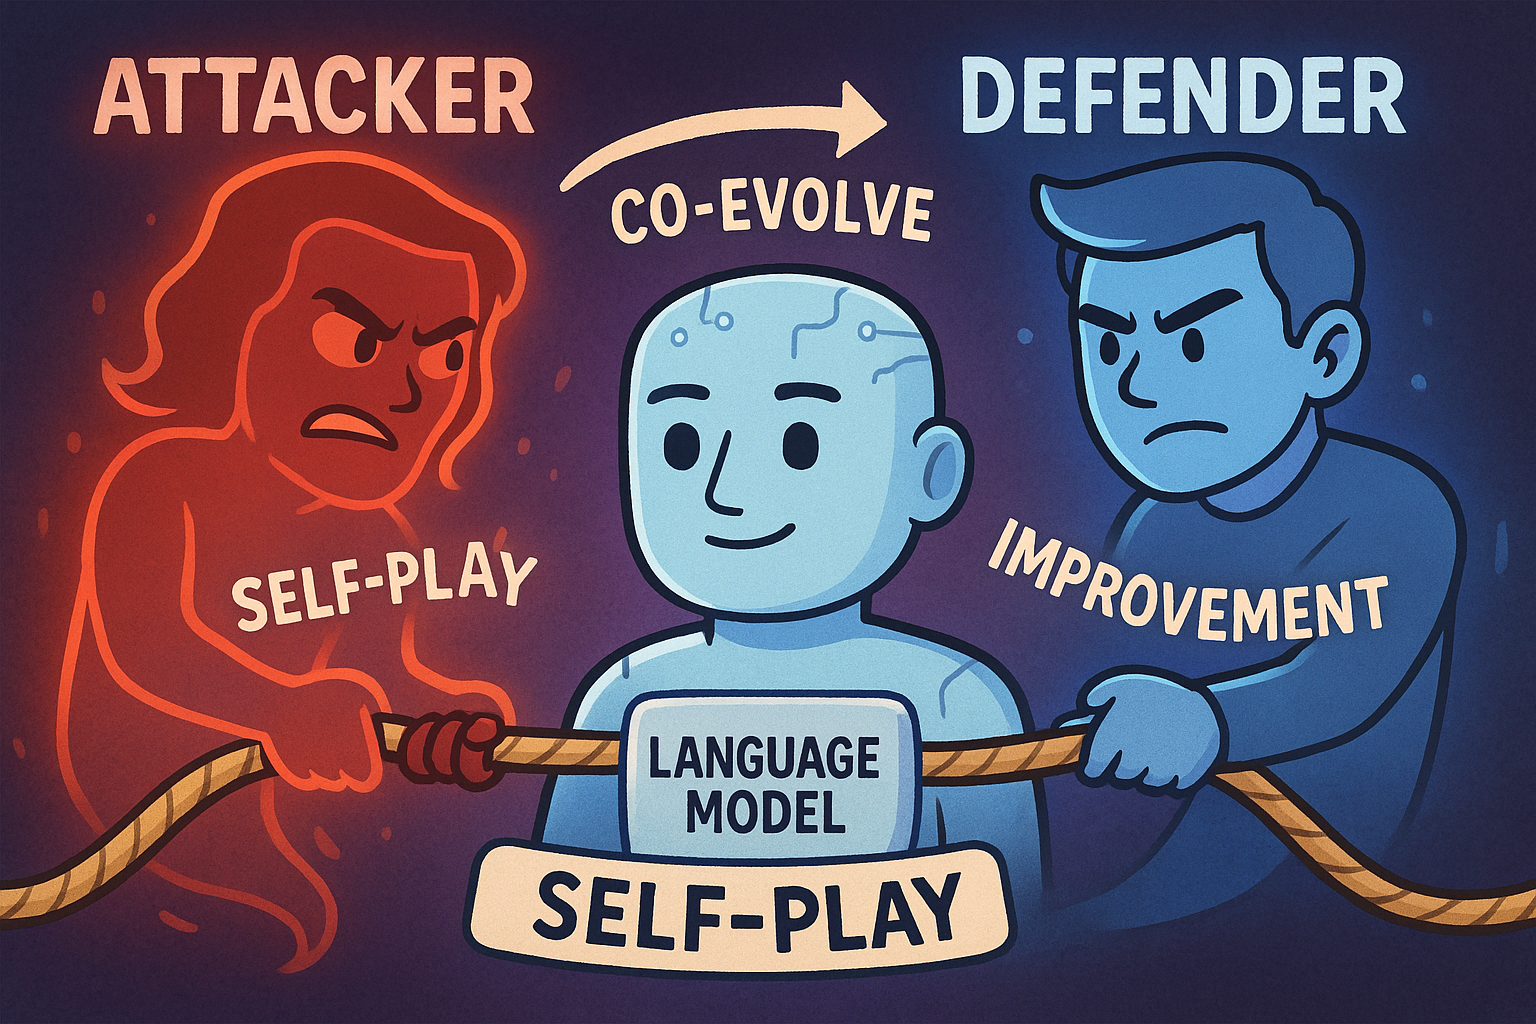
\includegraphics[width=6.0cm,height=3.5cm,keepaspectratio]{assets/selfplay-ideal.png}};
 \node at (11.85,4.9)
  {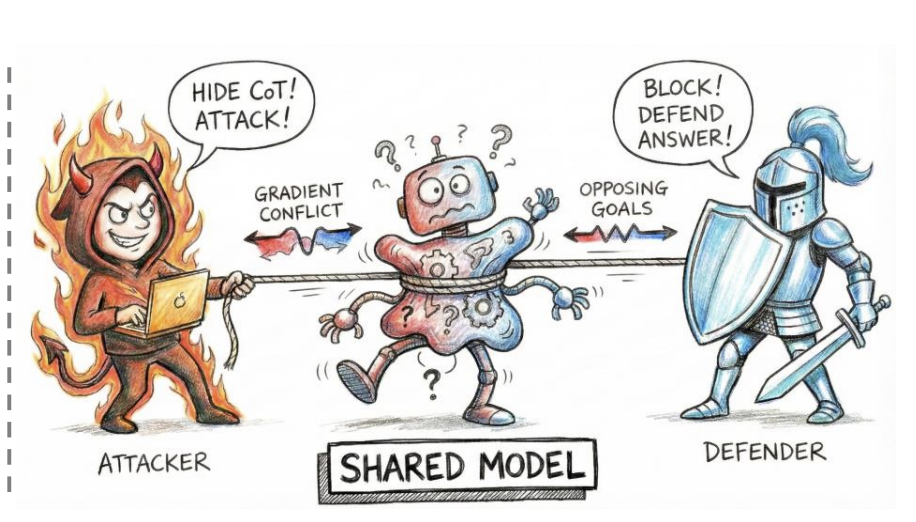
\includegraphics[width=6.5cm,height=3.5cm,keepaspectratio,
     trim=18bp 0 0 0,clip]{assets/selfplay-conflict.png}};
 \node[anchor=west,font=\normalsize\bfseries] at (.85,2.6) {Degenerate Solutions:};
 \node[anchor=west,font=\normalsize] at (5.0,2.6) {Attacker might \textbf{refuse to create attacks}};
 \node[anchor=west,font=\normalsize] at (5.0,1.95) {Defender \textbf{refuses all responses}};
\end{scope}
\end{tikzpicture}
